\documentclass[10pt,openany]{book}
 
\usepackage{geometry, graphicx, varioref, soul, verbatim, amsmath, calc, caption, wasysym, footmisc, makeidx, ifthen, subfigure, multicol, epstopdf, enumerate, wrapfig, textcomp, multirow, changepage, setspace, lscape, titlesec}
\usepackage[usenames,dvipsnames]{xcolor}  
\usepackage{mathrsfs}%for \mathscr
%\newcommand{\href}[2]{#2} \newcommand{\url}[1]{#1} \newcommand{\urlstyle}[1]{}

\definecolor{oiGA}{rgb}{0,0,0}
\definecolor{oiGB}{rgb}{.5,.5,.5}
\definecolor{oiGC}{rgb}{.85,.85,.85}
\definecolor{oiB}{rgb}{.337,.608,.741}
%\definecolor{oiB}{rgb}{0,0,0}
\definecolor{oiG}{rgb}{.298,.447,.114}
\definecolor{oiY}{rgb}{.957,.863,0}
\definecolor{oiR}{rgb}{.941,.318,.200}
\definecolor{redcards}{rgb}{.941,.318,.200}


\definecolor{rd}{rgb}{.80,.0,.0}
\definecolor{tableHL}{rgb}{.5,.1,.2}
\definecolor{tableHLBlue}{rgb}{.2,.4,.9}
\definecolor{highlight}{rgb}{.5,.1,.2}
\definecolor{highlightO}{rgb}{.1,.3,.8}
\definecolor{highlightT}{rgb}{.6,.3,.1}
\definecolor{ex}{rgb}{.0,.30,.55}
\definecolor{gray}{rgb}{.5,.5,.5}
\definecolor{steelBlue}{rgb}{.3,.4,.8}
\definecolor{excolor}{rgb}{.0,.3,.55}
\definecolor{secolor}{rgb}{.0,.3,.55}
\definecolor{comment}{rgb}{.65,.45,.25}
\definecolor{grayDark}{rgb}{.43,.43,.43}
\definecolor{grayLight}{rgb}{.65,.65,.65}
\definecolor{examplegray}{rgb}{0,0,0} %{.83,.83,.83}
\definecolor{termOColor}{rgb}{.65,.1,.1}



% _____ Online Version _____ %
\usepackage[bookmarksnumbered, colorlinks = false, pdfborder = {0 0 0}, urlcolor = oiGB, colorlinks=true, linkcolor = oiGB, citecolor = oiGB, backref = true]{hyperref}
\newcommand{\versiondate}[0]{February 21, 2019}
\newcommand{\printlocation}[0]{}

% _____ Print Version _____ %
%\definecolor{oiB}{rgb}{0,0,0}\usepackage[colorlinks=false,pdfborder={0 0 0},urlcolor= black,colorlinks=black,linkcolor=black, citecolor=black,backref=true]{hyperref}

% _____ COLOR PRINT Version _____ %
%\usepackage[colorlinks=false,pdfborder={0 0 0},urlcolor= black,colorlinks=black,linkcolor=black, citecolor=black,backref=true]{hyperref} \renewcommand{\printlocation}[0]{\noindent Printed in China. \\}

%bjoern start

\usepackage{pgfplots}


\usepackage{amsthm,amssymb}
\newtheorem{thm}{Theorem}[chapter]
\newtheorem{cor}[thm]{Corollary}
\newtheorem{lem}[thm]{Lemma}
\newtheorem{pro}[thm]{Proposition}
\newtheorem{nota}[thm]{Notation}
\newtheorem{con}[thm]{Conjecture}
\newtheorem{df}[thm]{Definition}
\newtheorem{rem}[thm]{Remark}
\newtheorem{exa}[thm]{Example}
\usepackage{tikz}
\usetikzlibrary{arrows,automata, positioning}
\usetikzlibrary{decorations.pathmorphing}
\tikzset{snake it/.style={decorate, decoration=snake}}
\newcommand{\abs}[1]{\lvert#1\rvert}

\DeclareMathOperator*{\argmax}{arg\,max}
\DeclareMathOperator*{\argmin}{arg\,min}

\DeclareMathOperator{\Var}{Var}
\DeclareMathOperator{\E}{\mathbb E}
\DeclareMathOperator{\SE}{SE}
\DeclareMathOperator{\SD}{SD}
\DeclareMathOperator{\AIC}{AIC}
\DeclareMathOperator{\BIC}{BIC}
\DeclareMathOperator{\TSS}{TSS}
\DeclareMathOperator{\ESS}{ESS}
\DeclareMathOperator{\RSS}{RSS}
\DeclareMathOperator{\TMS}{TSS}
\DeclareMathOperator{\EMS}{EMS}
\DeclareMathOperator{\RMS}{RMS}
\DeclareMathOperator{\slope}{slope}
\DeclareMathOperator{\intercept}{intercept}
\DeclareMathOperator{\vari}{var}
\DeclareMathOperator{\cov}{cov}
\renewcommand{\P}{\mathbb P}
\newcommand{\sheets}[1]{
\begin{quote}
\texttt{#1}
\end{quote}
}
%bjoern end


\usepackage[style=authortitle-ibid, maxnames=2,natbib=true,sortcites=true,block=space,backend=bibtex]{biblatex}
\bibliography{eoce.bib}

%EITHER:
%\makeindex
%OR:
\usepackage{imakeidx}
\makeindex[intoc]



% 1 Page Parameters
% 2 Special Commands for Editions
% 3 Content Modifications
% 4 Counters and Parameters
% 5 Section Coloring
% 6 Utilities
% 7 
% 8 Figures and Captions
% 9 Examples and Exercises
% 10 Special Boxes



%-------------------------------------------------------------
% 1 Page Parameters
% 1.1 Amazon
\setlength\paperheight{10in}
\setlength\textheight{8.25in}
\setlength\paperwidth{8in}
\setlength\textwidth{5.45in}
\setlength\voffset{-10mm}
% 1.2 Margin Size
% 1.2.1 Slim
%\setlength\hoffset{0.25in}
%\setlength\oddsidemargin{0.25in}
%\setlength\evensidemargin{0in}
% 1.2.2 Medium
\setlength\hoffset{3.7mm}
\setlength\oddsidemargin{3mm}
\setlength\evensidemargin{3mm}
% 1.2.3 Wide
%\setlength\hoffset{-5mm}
%\setlength\oddsidemargin{0.5in}
%\setlength\evensidemargin{0.5in}
% 1.3 PDF Parameters
%\setlength\paperheight{11in}
%\setlength\textheight{8.25in}
%\setlength\paperwidth{8.5in}
%\setlength\textwidth{5.45in}
%\setlength\voffset{-10mm}
%\setlength\oddsidemargin{0.75in}
%\setlength\evensidemargin{0.75in}
% 1.4 Margin Spacing
\setlength{\marginparsep}{5mm}
\setlength{\marginparwidth}{20mm}


% Tablet Version
%\setlength\paperheight{8.82in}\setlength\textheight{8.25in}\setlength\paperwidth{5.7in}\setlength\textwidth{5.45in}\setlength\voffset{-23.5mm}\setlength\hoffset{-27mm}\setlength\oddsidemargin{5mm}\setlength\evensidemargin{5mm}\setlength{\marginparsep}{5mm}\setlength{\marginparwidth}{35mm}




%-------------------------------------------------------------
% 2 Special Commands for Editions
\newcommand{\vspaceB}[1]{\vspace{#1}}
\newcommand{\hspaceB}[1]{\hspace{#1}}
\newcommand{\textB}[1]{}
\newcommand{\textC}[1]{#1}



%-------------------------------------------------------------
% 3 Content Modifications
\newcommand{\APVersion}[2]{#2}
\newcommand{\MultipleRegression}[2]{#1}
\newcommand{\MultipleRegressionChapter}[2]{#1}
\newcommand{\SimulationAndRandomization}[1]{#1}
\newcommand{\ANOVASection}[2]{#1}
\newcommand{\GLMSection}[2]{#1}




%-------------------------------------------------------------
% 4 Counters and Parameters
% 4.1 Counters
\newcounter{alwaysOne}
\setcounter{alwaysOne}{1}
\newcounter{alwaysTwo}
\setcounter{alwaysTwo}{2}
\newcounter{alwaysThree}
\setcounter{alwaysThree}{3}
\newcounter{alwaysFour}
\setcounter{alwaysFour}{4}
\newcounter{withinChNum}[chapter]
\setcounter{withinChNum}{0}
\newcounter{eoce}[chapter]
\renewcommand{\theeoce}{\arabic{chapter}.\arabic{eoce}}
\newcounter{eocesolch}
\setcounter{eocesolch}{0}
\newcounter{eocesol}[eocesolch]
\renewcommand{\theeocesol}{\arabic{eocesolch}.\arabic{eocesol}}
% 4.2 Parameters
\newlength{\exampleAboveBar}
\newlength{\exampleBelowBar}
\setlength{\exampleAboveBar}{-3.15mm}
\setlength{\exampleBelowBar}{-1.15mm}
% 4.3 Chapter Declarations
\newcommand\includechapter[2]{
  \setcounter{chapter}{#1}
  \addtocounter{chapter}{-1}
  \normalsize
  \include{#2/TeX/#2}
  \include{#2/TeX/#2_ex}}



%-------------------------------------------------------------
% 5 Section Coloring
% 5.1 Chapter
\titleformat{\chapter}[display]
{\color{oiB}\normalfont\huge\bfseries\raggedright}{\chaptertitlename\
\thechapter}{20pt}{\Huge}
% 5.2 Section
\titleformat{\section}
{\color{oiB}\normalfont\Large\bfseries}
{\color{oiB}\thesection}{1em}{}
% 5.3 Subsection
\titleformat{\subsection}
{\color{oiB}\normalfont\large\bfseries}
{\color{oiB}\thesubsection}{1em}{}


%-------------------------------------------------------------
% 6 Utilities
% 6.1 Helpful Editing Commands
\newcommand\Add[1]{\marginpar[{\Huge\color{oiR}$\bullet$}]{\Huge\color{oiR}$\bullet$}{\color{oiB}#1}}
\newcommand\Cut[1]{\marginpar[{\Huge\color{oiR}$\bullet$}]{\Huge\color{oiR}$\bullet$}{\color{oiGC}#1}}
\newcommand\Comment[1]{\marginpar[{\Huge\color{oiR}$\bullet$}]{\Huge\color{oiR}$\bullet$} {\color{oiG}{[#1]}}}
\newcommand{\note}[1]{\Comment{#1}}
% 6.2 Special Symbols
\newcommand{\degree}{\ensuremath{^\circ}}
% 6.3 Text Commands (Terms, Data, Variable, Response)
\newcommand{\term}[1]{\textbf{#1}\index{#1|textbf}}
\newcommand{\termsub}[2]{\textbf{#1}\index{#2|textbf}}
\newcommand{\termni}[1]{\textbf{#1}}
\newcommand{\hiddenterm}[1]{#1\index{#1|textbf}}
\newcommand{\indexthis}[2]{#1\index{#2}}
\newcommand{\termO}[1]{\textbf{\color{termOColor}#1}}
\newenvironment{data}[1]{\texttt{#1}}{}
\newenvironment{var}[1]{\texttt{#1}}{}
\newenvironment{resp}[1]{\texttt{#1}}{}
\newenvironment{calctext}[1]{{\color{oiB}\texttt{#1}}}{}
\newenvironment{calctextmath}[1]{{\color{oiB}\mathtt{#1}}}{}
\newenvironment{calcbutton}[1]{{\color{oiB}\texttt{#1}}}{}
% 6.4 Highlighting
\newenvironment{highlight}{\textbf}{}
\newcommand{\highlightO}[1]{\textbf{\color{oiB}#1}}
\newcommand{\highlightT}[1]{\emph{\color{oiR}#1}}
% 6.5 Lengths
\setlength{\parindent}{0.3in}
% 6.6 Hyperreferences
\newcommand{\urlwofont}[1]{\urlstyle{same}\url{#1}}
\newcommand{\oiRedirect}[2]{\href{http://www.openintro.org/redirect.php?go=#1&referrer=os3_pdf}{#2}}
\newcommand{\videoicon}[1][4.5mm]{
\includegraphics[height=#1]{extraTeX/icons/video_camera}~}
\newcommand{\CalculatorVideos}[1]{\begin{tipBox}{\tipBoxTitle[\videoicon]{Calculator videos}
Videos covering #1 using TI and Casio graphing calculators are available at \mbox{\oiRedirect{textbook-openintro_videos}{openintro.org/videos}}.}
\end{tipBox}}
\newcommand{\videohref}[2][4.5mm]{\oiRedirect{#2}{\raisebox{-0.3mm}[0pt]{
\includegraphics[height=#1]{extraTeX/icons/video_camera}}}}
\newcommand{\slideshref}[2][4.5mm]{\oiRedirect{#2}{\raisebox{-0.3mm}[0pt]{
\includegraphics[height=#1]{extraTeX/icons/slides}}}}
\newcommand{\videomarginhref}[2][4mm]{\oiRedirect{#2}{\raisebox{-3mm}[0pt]{
\includegraphics[height=#1]{extraTeX/icons/video_camera}}}}
\newcommand{\sectionvideohref}[2][6mm]{\oiRedirect{#2}{\raisebox{-0.5mm}[0pt]{
\includegraphics[height=#1]{extraTeX/icons/video_camera}}}}
\newcommand{\sectionslideshref}[2][6mm]{\oiRedirect{#2}{\raisebox{-0.5mm}[0pt]{
\includegraphics[height=#1]{extraTeX/icons/slides}}}}
\newcommand{\MarginVideo}[1]{\marginpar[{\videomarginhref{#1}}]{{\videomarginhref{#1}}}}



%-------------------------------------------------------------
% 7 



%-------------------------------------------------------------
% 8 Figures and Captions
% 8.1 & 8.2 Table & Figure Numbering
% Thanks @Herbert on StackExchange for helping clean up this style code!
% http://tex.stackexchange.com/questions/176978/latex-numbering-in-counters-appears-to-have-changed/177045?noredirect=1#comment409945_177045
\makeatletter
\let\c@table\c@figure
\makeatother
% 8.3 Caption Width
\newlength{\mycaptionwidth}
\setlength{\mycaptionwidth}{0.825\textwidth}
\setlength{\captionwidth}{\mycaptionwidth}




%-------------------------------------------------------------
% 9 Examples and Exercises
% 9.1 Exercises, within the text
% 9.1.1 Exercise Environment
\newcommand{\excolor}[1]{{\color{excolor}#1}}
\newenvironment{exercise}
{
\begin{itemize}\item[\color{oiB}$\bigodot$]\refstepcounter{equation}\noindent\normalsize\textbf{\color{oiB}Guided Practice \theexercise}\hspace{3mm}}
{\normalsize

\addvspace{3mm}
\end{itemize}}
% 9.1.2 Exercise Fine Tuning
\newcommand\theexercise{\thechapter.\arabic{equation}}
% 9.2 Examples
% 9.2.1 Example Environment
\newcommand\theexample{\thechapter.\arabic{equation}}
\newenvironment{example}[1]
{\begin{itemize}
\item[\color{oiB}\Large$\CIRCLE$]\refstepcounter{equation}\noindent\textbf{\color{oiB}Example \theexample}\hspace{0.3cm}#1\vspace{\exampleAboveBar}

{\color{examplegray}\rule{20mm}{0.1mm}}

\vspace{\exampleBelowBar}

\normalsize}{

\end{itemize}
\addvspace{3mm}
}
% 9.3 EOCEs: End of Chapter Exercises
% 9.3.1 Environment
\newenvironment{eoce}[2][]
{\refstepcounter{eoce}\noindent\small\textbf{\textcolor{oiB}{{\hypersetup{linkcolor=oiB}\ref{eoce_sol_\arabic{chapter}_\arabic{eoce}}}\label{eoce_\arabic{chapter}_\arabic{eoce}}}}\hspace{2mm} #1#2

\addvspace{3mm}

}
%{\em #2 } $\:$ \\ }
{}
% 9.3.2 EOCE Solutions
\newcommand{\eocesolch}[1]{
\refstepcounter{eocesolch}\noindent\textbf{\color{oiB}\arabic{eocesolch}\hspace{2mm}#1}

\addvspace{2mm}

}
{
\newcommand{\eocesol}[1]{\refstepcounter{eocesol}\noindent\textbf{\color{oiB}{\hypersetup{linkcolor=oiB}\ref{eoce_\arabic{eocesolch}_\arabic{eocesol}}}\label{eoce_sol_\arabic{eocesolch}_\arabic{eocesol}}}\hspace{2mm}{\small#1}\makebox[0pt]{\color{white}\tiny \refstepcounter{eocesol}\label{eoce_sol_\arabic{eocesolch}_\arabic{eocesol}}}

\addvspace{1mm}

}
% 9.3.3 EOCE Utilities
\newcommand{\qt}[1]{\textcolor{oiB}{\textbf{#1.}}}
\newcommand{\qtq}[1]{\textcolor{oiB}{\textbf{#1?}}}
\newcommand{\ec}[1]{\textcolor{oiB}{\footnotesize{~(#1)}}}% 9.3.4 EOCE Roman Parts
\newenvironment{romanparts}{
\begin{enumerate}[I.]
\setlength{\itemsep}{0mm}
}{\end{enumerate}}
% 9.3.5 EOCE Parts
\newenvironment{parts}{
%\vspace{-0.25cm}
\begin{enumerate}[(a)]
\setlength{\itemsep}{0mm}}
{\end{enumerate}}
% 9.3.6 EOCE Subparts
\newenvironment{subparts}{
\begin{enumerate}[i.]
\setlength{\itemsep}{0mm}}
{\end{enumerate}}
% 9.3.7 EOCE hyp environment
\newenvironment{hyp}{
\begin{itemize}
\setlength{\itemsep}{0mm}
}
{\end{itemize}
}
% 9.3.8 cond environment
\newenvironment{cond}{
\begin{enumerate}[1.]
\setlength{\itemsep}{0mm}
}
{\end{enumerate}
}




%-------------------------------------------------------------
% 10 Special Boxes
% 10.1 Term Box
\newcommand\tBoxTitleBuffer{\\[1.5mm]}
\newenvironment{tBoxTitle}[2][\tBoxTitleBuffer]{\textbf{\color{oiB}#2} #1
}{}
\newenvironment{termBox}[1]{
\addvspace{4mm}
\noindent{\color{oiB}\framebox[\textwidth][c]{\framebox[\textwidth-3mm][l]{ \\
	\vspace{0.5cm} \\
	\begin{minipage}[b]{\textwidth-3mm}
		\begin{minipage}[t]{2mm}
			\hspace{2mm}
		\end{minipage}
		\begin{minipage}[b]{\textwidth-10mm}
			\color{black}\ \\[-0.7mm]
			#1
			
			\vspace{1mm}
		\end{minipage}
	\end{minipage}}}}
}{

\addvspace{1mm}}
% 10.2 Tip Box
\newenvironment{tipBoxTitle}[2][TIP:\ ]{\textbf{\color{oiB}#1#2}\\[0.3mm]}{}
\newenvironment{tipBox}[1]{
\addvspace{4mm}
\noindent{\color{oiB}\framebox[\textwidth][l]{ \\
	\vspace{5mm} \\
	\begin{minipage}[b]{\textwidth-4mm}
		\begin{minipage}[t]{2mm}
			\hspace{2mm}
		\end{minipage}
		\begin{minipage}[b]{\textwidth-8mm}
			\color{black}\ \\[-0.7mm]
			#1
			
			\vspace{1mm}
		\end{minipage}
	\end{minipage}}}
}{

\addvspace{1mm}}
% 10.3 Caution Box
\newenvironment{caution}[2]{
\addvspace{4mm}
\noindent{\color{oiB}\framebox[\textwidth][l]{ \\
	\vspace{5mm} \\
	\begin{minipage}[b]{\textwidth-4mm}
		\begin{minipage}[t]{2mm}
			\hspace{2mm}
		\end{minipage}
		\begin{minipage}[b]{\textwidth-8mm}
			\textbf{\color{oiB}Caution: #1} \\[1mm]
			\color{black}#2
		\end{minipage}
	\end{minipage}}}
}{

\addvspace{1mm}}







%
% Tablet Version
\setlength\paperheight{8.82in}
\setlength\textheight{8.25in}
\setlength\paperwidth{5.7in}
\setlength\textwidth{5.45in}
\setlength\voffset{-23.5mm}
\setlength\hoffset{-27mm}
\setlength\oddsidemargin{5mm}
\setlength\evensidemargin{5mm}
\setlength{\marginparsep}{5mm}
\setlength{\marginparwidth}{35mm}

 %uncomment to make a tablet version. The tablet version doesn't have the margin notes

\title{\huge Statistics for Calculus Students\vspace{1.5mm} %\\ \Large Random forest, hidden Markov
}
\author{Bj\o rn Kjos-Hanssen \\
\small\emph{Professor} \\
\small\emph{University of Hawai\textquoteleft i at M\=anoa} \\
\vspace{6mm}%
\small\emph{bjoernkh@hawaii.edu} \\
Samuel D.~Birns \\
\small\emph{Data Scientist} \\
\small\emph{Coalition, Inc.} \\
\vspace{6mm}%
\small\emph{sbirns@hawaii.edu}}
%_derivative}
\date{}
\setcounter{tocdepth}{1}

\begin{document}
\renewcommand{\thepage}{}
\maketitle
\chapter*{}
\vfill

\noindent Copyright $\copyright$ 2019. First Edition. \\
Updated: \versiondate. \\

\noindent
\includegraphics[width=.7in]{extraTex/preamble/88x31.png}

\noindent This textbook is available under a Creative Commons BY-SA 3.0 license.

\noindent Visit 

\noindent\url{http://math.hawaii.edu/wordpress/open-educational-resources/}

\noindent for a free PDF and more information.\\ %to download the textbook's source files, or for more information about the license. \\
\printlocation

%\noindent Modified versions of this textbook, including reformatted electronic versions, may not be redistributed under a title that suggests association with or endorsement by OpenIntro, e.g. it cannot be titled \emph{OpenIntro Statistics}. %More information on branding restrictions for derivatives is available on the Rights page at~\href{http://www.openintro.org/rights.php}{openintro.org}.

%_derivative}
\renewcommand{\thepage}{\arabic{page}}
\tableofcontents
\chapter*{Preface}

This book is a supplement to OpenIntro Statistics, which may be downloaded as a free PDF at \oiRedirect{textbook-openintro}{\color{black}\textbf{openintro.org}}. \vspace{3mm}


\noindent By choosing the title \emph{Statistics for Calculus Students} we intended to summarize the following prerequisite situation.\vspace{-1mm}
\begin{enumerate}
\setlength{\itemsep}{0mm}
\item[(1)] Students should have studied some calculus, say Calculus 1 and 2.
\item[(2)] Students could still be studying Calculus --- for instance, Calculus 3 (multivariable) is not assumed.
\item[(3)] Although it is essential for a full understanding of statistics, \emph{linear algebra} is not required to read this book.
\end{enumerate}
In particular, the book is designed to be appropriate for MATH 372 (Elementary Probability and Statistics) at University of Hawai\textquoteleft i at M\=anoa.

\noindent This is not a textbook on probability. While we review some basic concepts, we assume that students have some knowledge of probability as can be gained through Chapters 1--9 of Grinstead and Snell's \emph{Introduction to Probability}\footnote{Free download available at \url{http://www.dartmouth.edu/~chance/teaching_aids/books_articles/probability_book/amsbook.mac.pdf}.}.
Thus, we assume the student has seen some single-variable calculus-based probability, and some algebra-based statistics; and we intend to bridge the gap to single-variable calculus-based statistics.

\subsection*{Textbook overview}

The chapters of this book are as follows:
\begin{description}
\setlength{\itemsep}{0mm}
\item[1. Introduction to data.] Data structures, variables, summaries, graphics, and basic data collection techniques.
\item[2. Probability.] The basic principles of probability. %An understanding of this chapter is not required for the main content in Chapters~\ref{modeling}-\ref{multipleAndLogisticRegression}.
\item[3. Distributions of random variables.] Introduction to the normal model and other key distributions.
\item[4. Foundations for inference.] General ideas for statistical inference in the context of estimating the population mean.
\item[5. Inference for numerical data.] \hspace{1mm}Inference for one or two sample means using the \mbox{$t$-distribution}. %, and also comparisons of many means using ANOVA.
\item[6. Inference for categorical data.] Inference for proportions using the normal and $\chi^2$ distributions, as well as simulation and randomization techniques.
\item[7. Introduction to linear regression.] An introduction to regression with two variables. %Most of this chapter could be covered after Chapter~\ref{introductionToData}.
\item[8. Special topics.] Introduces maximum likelihood models and their applications to finding a hidden Markov model. Algebraic statistics, entropy, likelihood, Markov chains, and information criteria.
\end{description}

%\emph{OpenIntro Statistics} was written to allow flexibility in choosing and ordering course topics. The material is divided into two pieces: main text and special topics. The main text has been structured to bring statistical inference and modeling closer to the front of a course. Special topics, labeled in the table of contents and in section titles, may be added to a course as they arise naturally in the curriculum.


%\subsection*{Videos for sections and calculators}

%The \videohref[4mm]{textbook-openintro_videos} icon indicates that a section or topic has a video overview readily available. The~icons are hyperlinked in the textbook PDF, and the videos may also be found at
%\begin{center}
%\oiRedirect{textbook-openintro_videos}{\color{black}\textbf{www.openintro.org/stat/videos.php}}
%\end{center}


\subsection*{Examples, exercises, and appendices}

Examples and Guided Practice throughout the textbook may be identified by their distinctive bullets:

\begin{example}{Large filled bullets signal the start of an example.}
Full solutions to examples are provided and may include an accompanying table or figure.
 \end{example}

\begin{exercise}
Large empty bullets signal to readers that an exercise has been inserted into the text for additional practice and guidance. Students may find it useful to fill in the bullet after understanding or successfully completing the exercise. Solutions are provided for all Guided Practice in footnotes.\footnote{Full solutions are located down here in the footnote!}
\end{exercise}

There are exercises at the end of each chapter for practice or homework assignments. Odd-numbered exercise solutions are in Appendix~\ref{eoceSolutions}.

\subsection*{Google Sheets}
Occasional references to technology are made, in which cases our software of choice is \texttt{Google Sheets}. This choice was made on the basis of Google Sheets being freely available and only a few clicks away from University of Hawai\textquoteleft i students' Gmail accounts.

%\subsection*{OpenIntro, online resources, and getting involved}

%OpenIntro is an organization focused on developing free and affordable education materials. \emph{OpenIntro Statistics} is intended for introductory statistics courses at the college level. And this tome, \emph{Statistics for Calculus Students}, implies a college-level mathematics course.

%We encourage anyone learning or teaching statistics to visit \oiRedirect{textbook-openintro}{\color{black}\textbf{openintro.org}} and get involved. We also provide many free online resources, including free course software. 

%We value your feedback. If there is a particular component of the project you especially like or think needs improvement, we want to hear from you. You may find our contact information on the title page of this book or on the \oiRedirect{textbook-openintro_about}{About} section of \oiRedirect{textbook-openintro}{\color{black}\textbf{openintro.org}}.

\subsection*{Acknowledgements}

This project would not be possible without the passion and dedication of all those involved. %We hope you will join us in extending a \emph{thank you} to all the project volunteers.
The authors would like to thank faculty members in the Department of Mathematics at  University of Hawai\textquoteleft i at M\=anoa for their involvement and ongoing contributions. We~are also very grateful to the students who took our classes and provided us with valuable feedback over the last several years.

We are thankful to Outreach College at University of Hawai\textquoteleft i at M\=anoa for support under their Open Educational Resources grant program.

\subsection*{Second Edition}
This Second Edition is under development during Fall 2025 as part of the course MATH 372.

\normalsize

\includechapter{1}{ch_intro_to_data}
\includechapter{2}{ch_probability}
\includechapter{3}{ch_distributions}
\includechapter{4}{ch_inference_foundations}
\includechapter{5}{ch_inference_for_means}
\includechapter{6}{ch_inference_for_props}
\includechapter{7}{ch_regr_simple_linear}
\includechapter{8}{ch_markov}

\appendix
\chapter{End of chapter exercise solutions}
\label{eoceSolutions}



%_______________
\eocesolch{Introduction to data}



%_______________
\begin{multicols}{2}

% 1

\eocesol{(a)~Possible answers: $^1$Basically true. Categorical variables have no numerical meaning. Examples: Hair color, gender, field of study. $^2$As a kind of counterexample, consider something like \emph{What is your favorite number among $\sqrt 2$, $\sqrt{-1}$, and $\pi$?}
Here it doesn't make much sense to take the average of the responses, so it is not your typical numerical variable. But it does involve numbers.\\
(b)~Possible answers: $^1$Basically true. A discrete variable is a variable whose value is obtained by counting; a continuous variable is a variable whose value is obtained by measuring. %Thanks to Hau Nguyen.
$^2$As a kind of counterexample, consider a \emph{hybrid} variable $X$ which has a 50\% chance of $X=3$, and a 50\% of being a number $1\le X\le 2$, uniformly distributed (so that, given that $1\le X\le 2$, the probability that $X\le 5/4$ is 25\%, for instance).
(c)~Possible answers: $^1$Basically false. $^2$As a kind of counterexample, consider \emph{What is your favorite real number?} (where all real numbers are considered legitimate answers).
%\footnote{This is a solution to Exercise \ref{catcat}.}
}
% 3

\eocesol{(a)~New mean = 10+old mean $=70.7+10=80.7$.
(b)~New mean = $2\cdot$old mean $=70.7\cdot 2=141.4$. In formulae, $E(2X)=2E(X)=2(70.7)=141.4$ where $E(X)$ is the mean of $X$.
(c)~The means are
\begin{eqnarray*}
	&=&\frac{x_1+c_1+x_2+c_1+\dots+x_n+c_1}n\\
	&=&\frac{nc_1+ (x_1+\dots+x_n)}n=c_1+\frac{x_1+\dots+x_n}n.
\end{eqnarray*}
and $\frac{x_1c_2+\dots+x_nc_2}n=c_2\frac{x_1+\dots+x_n}n$, respectively.
In formulae, $E(X+c_1)=E(X)+c_1$ and $E(c_2X)=c_2E(X)$.
%\footnote{This is a solution to Exercise \ref{extra_mean}.}
\footnote{By the way, a solution to 1.2 is mean $=(55+59+64+68+70+70+71+76+76+98)/10$=70.7, median = (70+70)/2=70, mode = 70,76.}
}

\eocesol{This uses Jensen's Inequality, which says that if $f''(x)\ge 0$ for all $x$ (so $f$ is \emph{concave up} or \emph{convex}) then a chord drawn between two points on the graph of $f$ will lie above the graph of $f$. In symbols, $f(tx_1+(1-t)x_2)\le tf(x_1)+(1-t)f(x_2)$ for al l$0\le t\le 1$. By iterating, we get for $a+b+c=1$,
\begin{eqnarray*}
	&&f(ax+by+cz)\\
	&=&f\left(ax+(1-a)\left(\frac{b}{1-a}y + \frac{c}{1-a}z\right)\right)\\
	&\le&af(x)+(1-a)f\left(\frac{b}{1-a}y + \frac{c}{1-a}z\right)\\
	&\le&af(x)+(1-a)\left(\frac{b}{1-a}f(y) + \frac{c}{1-a}f(z)\right)\\
	&=&af(x)+bf(y)+cf(z)
\end{eqnarray*}
and similarly for $a_1+\dots+a_n=1$, $f(\sum a_ix_i)\le\sum a_if(x_i)$.
In particular, since the function $f(x)=-\ln x$ satisfies $f''(x)=1/x^2\ge 0$ in its domain $x> 0$, and taking each $a_i=1/n$, we have
\[
	-\ln(\overline x) \le \overline{-\ln x} := \frac1n \sum -\ln x_i,
\]
which gives the arithmetic-geometric inequality by raising $e$ to the power of both sides. For the harmonic inequality, consider instead
\[
	n/\sum(1/x_i)=\left(\sum (1/x_i)/n\right)^{-1}
\]
which reduces the problem to the arithmetic-geometric inequality with $x_i$ replaced by $1/x_i$.
%\footnote{This is a solution to Exercise \ref{harmonic}.}
}

\eocesol{(a)~Let $g(x)=f(x)+c$. Then
\begin{eqnarray*}
	\mathrm{avg}_{g}&=& \frac1{b-a}\int_a^b g(x)\,dx\\
	&=& \frac1{b-a}\int_a^b f(x)+c\,dx = \mathrm{avg}_f + c.
\end{eqnarray*}
(b)~Let $h(x)=c\cdot f(x)$. Then
\begin{eqnarray*}
	\mathrm{avg}_h &=& \frac1{b-a}\int_a^b h(x)\,dx\\
	&=& \frac1{b-a}\int_a^b c\cdot f(x)\,dx = c\cdot\mathrm{avg}_g.
\end{eqnarray*}
%\footnote{This is a solution to Exercise \ref{inv_ave}.}
\footnote{By the way, a solution to 1.8 is:
Since $f$ is continuous, then there exists some number $c$ such that $a<c<b$, and
\[
f'(c)=\frac{f(b)-f(a)}{b-a}=\frac{\int_a^b f'(x)\,dx}{b-a}.
\]
Let $g(x)=f'(x)$,then
\[
g(c)=\frac1{b-a}\int_a^b g(x)\,dx=\mathrm{avg}_g.
\]
}
}

\eocesol{We have $(\frac43)(\frac32)=2=2^{12/12}=2^{5/12}2^{7/12}$. The inequalities both follow from $2^{19}=524,288<531,441=3^{12}$.}
%_______________
\end{multicols}


%\textC{\newpage}


%_______________
\eocesolch{Probability}



%_______________
\begin{multicols}{2}

% 1

\eocesol{(a)~Use the substitution $u=(x-\mu)/\sigma$.
(b)~What we need to verify: for the mean, $\int x f(x)\,dx=\mu$ (use the substitution $u=x-\mu$ in the integral). For the median, $P(X\le\mu=1/2$. For the mode, $\varphi'(\mu)=0$.
(c)~The variance is $E(X^2)-E(X)^2$ so we need to evaluate $E(X^2)=\int x^2\varphi(x)\,dx$.
%\footnote{This is a solution to Exercise \ref{normal_dist}}
}

% 3


\eocesol{(a)~We have $\int f(x)\,dx=1$ using the derivative of $\arctan$.\\
(b)~The median and mode are both 0, by symmetry $f(x)=f(-x)$ and since $f'(x)\le 0$ if and only if $x\ge 0$.\\
(c)~Hint: the mean would be $\int xf(x)\,dx$ but this is similar to the harmonic series $\sum_n 1/n$. You can use the substitution $u=1+x^2$.\\ %Thanks to Hau
(d)~Since the mean does not exist, we cannot claim that sample averages $\overline x_n$ from this distribution will converge to the mean. (If the mean were $+\infty$ we could perhaps argue that sample averages would diverge to $+\infty$, but since $-\infty$ is equally plausible as a mean here, all we can expect is ``chaos'' in the behavior of $\overline x_n$.
%\footnote{This is a solution to Exercise \ref{cauchy_dist}.}
}

%\eocesol{5\% increase in value.}
%\eocesol{5\% increase in value.}



%_______________
\end{multicols}



\newpage


%_______________
\eocesolch{Distributions of random variables}


\begin{figure}
\centering
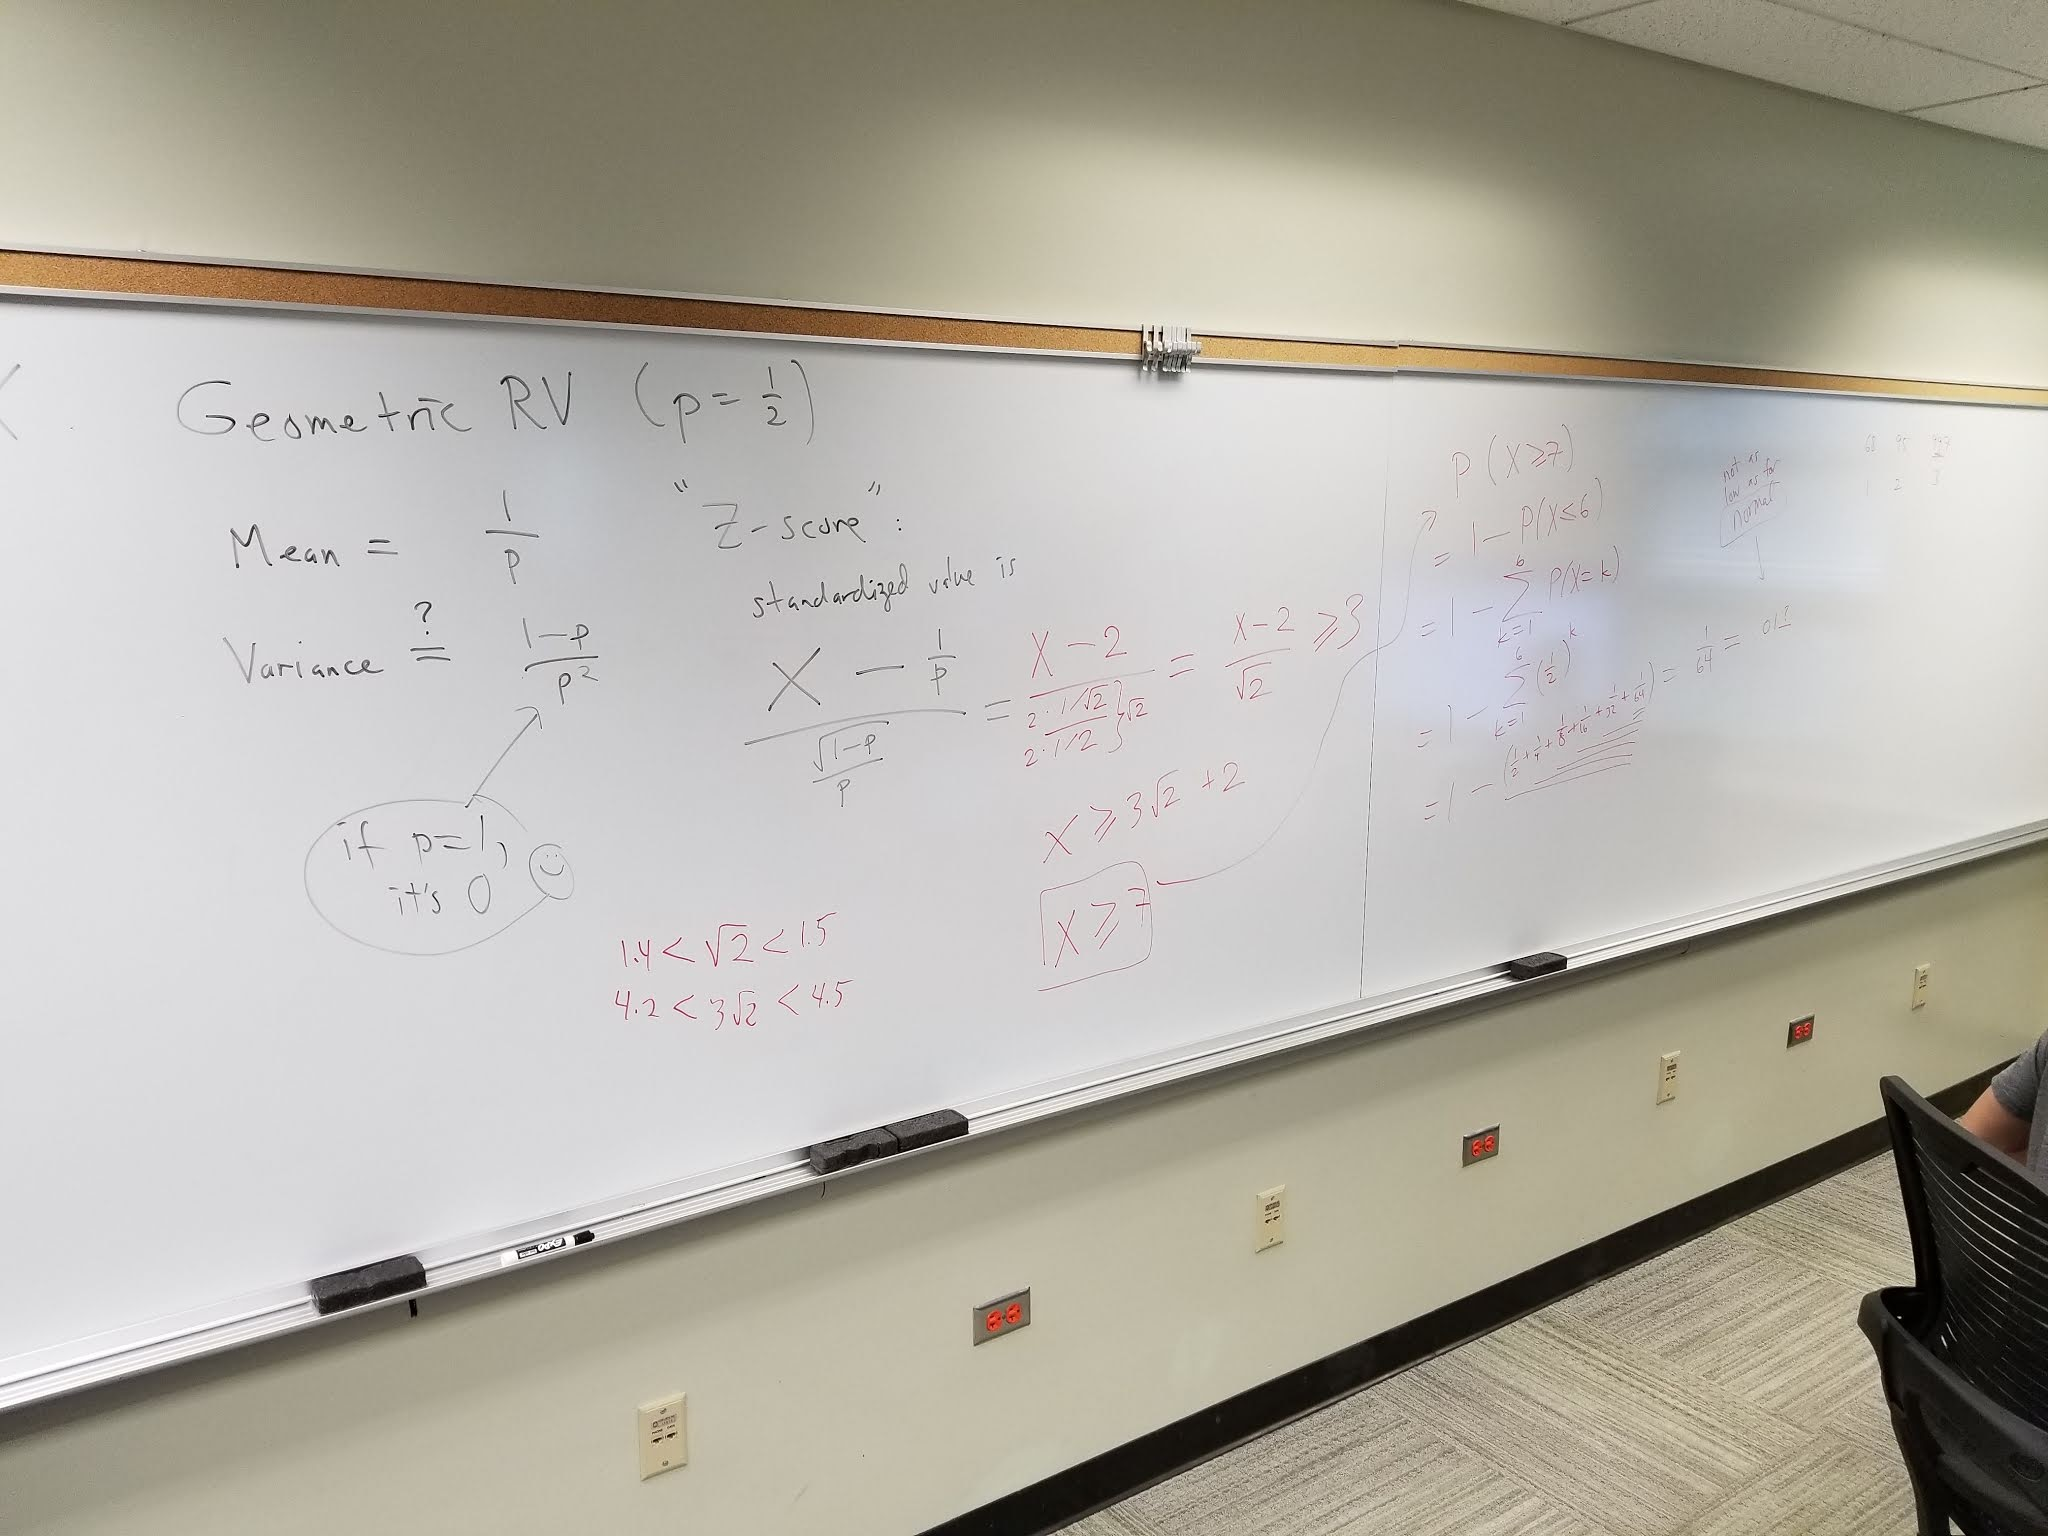
\includegraphics[width=5in]{extraTex/eoceSolutions/likelihoodprinciple}
\caption{A calculation related to the Likelihood Principle, from Fall 2018 in Webster Hall 101, UH M\=anoa campus.}\label{LP}
\end{figure}
%_______________
\begin{multicols}{2}

% 1

\eocesol{(a)~In general, normality is expected when dealing with variables for which the Central Limit Theorem holds approximately: sums of IID (independent, identically distributed) variables. A safe example is proportions of heads and tails when flipping a coin. Height of individuals may be an example if a person's height is approximately the result of a sum of independent events such as healthy meals, nights of sufficient sleep (for the individual or for their parents), etc.\\
(b)~This is a tricky one; a library deep-dive into the given article is probably your best bet.\\
(c)~We assume the student can look up things like \emph{power-law distribution} online. One example is then \emph{the frequencies of words in most languages}.
%\footnote{This is a solution to Exercise \ref{skewed_but_real}.}
\footnote{And here is a solution to 3.2 Three Sigma: (a)~$P(X=3)=0.5(1-0.5)3-1=0.125=12.5\%$; $P(X=10)=0.5(1-0.5)10-1=0.00097=0.097\%$; $P(X=100)=0.5(1-0.5)100-1=0\%$.
(b)~$P(Z>3)=1-P(Z<3)=1-0.99865=0.00135$, $\implies$0.5(1-0.5)n-1=0.00135, $\implies n\ge 9.5$. However, interestingly, if we consider the geometric distribution instead we get a different answer. This relates to a famous discussion about the Likelihood Principle \url{https://en.wikipedia.org/wiki/Likelihood_principle} (see Figure \ref{LP}).}
}{}

% 3

\eocesol{(a)~This is just $P(X=k-1)$ where $X$ is binomial with parameters $p$ and $n-1$. To wit:
\begin{eqnarray*}
	&&\binom{n-1}{k-1} p^{k-1}(1-p)^{(n-1)-(k-1)}\\
	&=& \binom{n-1}{k-1} p^{k-1}(1-p)^{n-k}.
\end{eqnarray*}
(b)~Since the $n$th trial is independent of the previous trials, this is
\begin{eqnarray*}
	&&p\cdot \binom{n-1}{k-1} p^{k-1}(1-p)^{n-k} \\
	&=&\binom{n-1}{k-1} p^{k}(1-p)^{n-k}.
\end{eqnarray*}
(c)~The answer to (b) is exactly the probability that a negative binomial variable $Y$ with parameters $n$ and $p$ will take value $k$.
This is not surprising since the following two conditions are equivalent:
\begin{itemize}
\item the first success happens in trial $n$;
\item the first $n-1$ trials are failures and the $n$th trial is a success.
\end{itemize}
%\footnote{This is a solution to Exercise \ref{negative_binomial}.}
}

% 5
\eocesol{We solve for $\beta$:
\[
\beta=\frac{x}{1-x}\left(2\alpha+\frac1{1-x}\right)
\]
Then
\begin{eqnarray*}
E(X^2)&=&\sum_{k=1}^\infty k^2 P(X=k)\\
&=&\sum_{k=1}^\infty k^2 (1-p)^{k-1}p = \frac{p}{1-p}\sum_{k=1}^\infty k^2 (1-p)^k\\
&=& \frac{p}{1-p}\beta\\
&=& \frac{p}{1-p} \frac{1-p}{p} \left(2\frac{1-p}{p^2} +\frac1p\right)\\
&=& \frac{2-2p+p}{p^2} = \frac{2-p}{p^2}
\end{eqnarray*}
giving $\sigma^2 = \frac{2-p}{p^2}-(1/p)^2 = \frac{1-p}{p^2}$, as desired.
}{}

\end{multicols}
%_______________
\eocesolch{Foundations for inference}



%_______________
\begin{multicols}{2}

% 1

\eocesol{(a)~If you are wondering whether a certain drug helps to cure cancer, you are not interested in proving that the drug just changes the outcomes for cancer.
You really want it to help and not hurt. So a 1-sided test is appropriate.\\
(b)~If you are hoping that a certain coin is fair, you don't necessarily care in which direction it may be biased.
Too many heads and too many tails are not different outcomes for you, in any interesting sense. So you want a 2-sided test.}

% 3
\eocesol{(a)~If $X$ and $Y$ are independent then so are any deterministic (not random) functions of them $f(X)$, $g(Y)$. 
Moreover, whenever $U$ and $V$ are independent then $E(UV)=E(U)E(V)$. These facts are proved in more advanced texts.
In particular, for any constant $t$, $e^{tX}$ and $e^{tY}$ are independent, and
\begin{eqnarray*}
	M_{X+Y}(t)&=&E(e^{t(X+Y)}) = E(e^{tX}e^{tY})\\
	 &=& E(e^{tX})E(e^{tY}) = M_X(t)M_Y(t).
\end{eqnarray*}
The other part is easier:
\[
	M_{cX}(t)=E(e^{t(cX)}) = E(e^{(ct)X}) = M_X(ct).
\]
(b)~The power series of $e^x$ is $\sum x^n/n!$. Now assuming that $E(\sum)=\sum(E)$ (proved in advanced real analysis texts),
\begin{eqnarray*}
	M_X(t)=E(e^{tX}) &=& E\left(\sum (tX)^n/n!\right)\\
	 &=& \sum E(X^n)t^n/n!
\end{eqnarray*}
(c)~We have
\[
	M^{(n)}_X(0)= \frac{d^n}{dt^n}M_X(t)\bigg|_{t=0}.
\]
We then use $d/dt\sum^{\infty} = \sum^{\infty}d/dt$ (proved in advanced real analysis texts), and
\[
	\frac{d^n}{dt^n}t^n\bigg|_{t=0}=n!
\]
to finish.}

% 5
\eocesol{%(a)~easy\\
%(b)~nice.\\
%(c)~nice.\\
(d)~Suppose they are all bounded by $b$.\\
(e)~We use the fact that the normal distribution with mean $\mu$ and variance $\sigma^2$ is the only distribution whose cumulants are $\mu,\sigma^2,0,0,0,\dots$.}

\end{multicols}


\newpage

\eocesolch{Inference for numerical data}

%%%%%%%%%%%%%%%%%%%%%%%%%%%%%

\begin{multicols}{2}

% 1
\eocesol{The price of \emph{Statistics for Calculus Students} printed and bound, in the UCLA bookstore and on Amazon, is an example of paired data. The price of \emph{Stats: Data and Models} by de Veaux, at UCLA, and \emph{Probability: theory and examples} by Durrett, on Amazon, is an example of unpaired data.}

\eocesol{(a)~We are selecting a substantial proportion of the homes. Let's say we look at the proportion who plan to vote for the Democratic candidate (or, alternatively, the Republican candidate). If the sample was small compared to the population, but still large in absolute terms, we could argue that we have a sampling distribution to which the Central Limit Theorem applies. But 20\% is too large a sample, creating dependencies. For instance, if all of the first 10\% vote Republican it becomes unlikely that many of the other 10\% vote Democrat. \\
(b)~Now the proportion of homes selected is small enough for most purposes. However, the sample size of 10 is a bit small for the normal approximation to be reliable.}

% 3
\end{multicols}
% Chp 6
\eocesolch{Inference for categorical data}

%%%%%%%%%%%%%%%%%%%%%%%%%%%%%

\begin{multicols}{2}

% 1
\eocesol{(a)~A hint is already given.\\
(b)~We have
\[
	\Gamma(1/2) = \int_0^\infty t^{1/2-1} e^{-t}\,dt = \int_0^\infty \frac{dt}{e^t\sqrt{t}}.
\]
Now try the substitution $t=u^2/2$.}

\eocesol{Note that there are some ``easy'' solutions that don't quite work. But moment generating functions can be used:
\[
	M_{X_1+X_2}(t) = M_{X_1}(t) M_{X_2}(t)
\]
Solve for $M_{X_2}(t)$.}

% 3
\eocesol{Squaring both sides, %\begin{eqnarray*}
%	\sqrt{(\hat p_y(1-\hat p_y)/1924)+(\hat p_x(1-\hat p_x)/3666)} &=& 0.01\\
%	\hat p_y-\hat p_x&=&0.04
%\end{eqnarray*}
\begin{eqnarray*}
	\frac{\hat p_y(1-\hat p_y)}{1924}+\frac{\hat p_x(1-\hat p_x)}{3666} &=& 10^{-4}\\
	\hat p_y-\hat p_x&=&\frac1{25}
\end{eqnarray*}
\begin{eqnarray*}
	\frac{(\hat p_x+\frac1{25})(1-\hat p_x-\frac1{25})}{1924}+\frac{\hat p_x(1-\hat p_x)}{3666} &=& 10^{-4}
\end{eqnarray*}
\[
	\frac{(u+\frac1{25})(1-u-\frac1{25})}{1924}+\frac{u(1-u)}{3666} = 10^{-4}
\]
This we can solve by hand; Wolfram Alpha gives\footnote{\url{https://www.wolframalpha.com/input/?i=\%5Cfrac\%7B(u\%2B\%5Cfrac1\%7B25\%7D)(1-u-\%5Cfrac1\%7B25\%7D)\%7D\%7B1924\%7D\%2B\%5Cfrac\%7Bu(1-u)\%7D\%7B3666\%7D+\%3D+10\%5E\%7B-4\%7D}}
$u = 5093/10750 - \sqrt{7133687/2}/5375$, i.e., $u\approx 0.12240$ or $u\approx 0.82514$.
Looking at the paper \footnote{\url{http://thegeeksverse.com/wp-content/uploads/2014/09/SexOrColorPref.pdf}}, we see that actually
$p_y=233/1924=.1211$ and $p_x=306/3666=.0835$ which gives the standard error $0.0087\approx 0.01$.
%\footnote{This is a solution to Exercise \ref{zain_email}.}
}

\end{multicols}

\newpage

\eocesolch{Introduction to linear regression}

\begin{multicols}{2}

% 1
\eocesol{(a)~The points $\{(0,0),(1,1),(2,2)\}$ form one example. We need at least 3 points for $r$ to be defined because of the $n-2$ in a denominator.\\
(b)~Using
\[
r =\frac{\sum ^n _{i=1}(x_i - \bar{x})(y_i - \bar{y})}{\sqrt{\sum ^n _{i=1}(x_i - \bar{x})^2} \sqrt{\sum ^n _{i=1}(y_i - \bar{y})^2}}
\]
When $n=0$ or $n=1$, we have all $x_i=\bar{x}$ and $y_i=\bar{y}$, hence $r$ is of the form ``$0/0$'' and undefined.
When $n=2$, $x_1-\bar{x}=x_1-\frac{x_1+x_2}2 = \frac{x_1-x_2}2$ and
\begin{eqnarray*}
r &=&\frac{\frac{x_1 - x_2}2 \frac{y_1-y_2}2 + \frac{x_2-x_1}2\frac{y_2-y_1}2}{\sqrt{2((x_1-x_2)/2)^2 2((y_1-y_2)/2)^2}}\\
&=&\frac{\frac{x_1 - x_2}2 \frac{y_1-y_2}2 + \frac{x_2-x_1}2\frac{y_2-y_1}2}{2\sqrt{((x_1-x_2)/2)^2 ((y_1-y_2)/2)^2}}\\
&=&2\frac{\frac{x_1 - x_2}2 \frac{y_1-y_2}2 + \frac{x_2-x_1}2\frac{y_2-y_1}2}{\sqrt{((x_1-x_2))^2 ((y_1-y_2))^2}}\\
&=&\frac{(x_1-x_2)(y_1-y_2)}{\abs{(x_1-x_2)(y_1-y_2)}}\\
&=&\mathrm{sign}((x_1-x_2)(y_1-y_2)),
\end{eqnarray*}
where
\[
\mathrm{sign}(x)=
\begin{cases}
1& \text{if }x>0,\\
-1&\text{if }x<0,\\
\text{undefined}&\text{if }x=0.
\end{cases}
\]
In any case, this is a long-winded way of saying that there can be no example with $n=2$, either.
How about $n=3$? We get the algebraic equation
\begin{eqnarray*}
&&   (2x_1-x_2-x_3)(2y_1-y_2-y_3)\\
&+& (2x_2-x_3-x_1)(2y_2-y_3-y_1)\\
&+& (2x_3-x_1-x_2)(2y_3-y_1-y_2) = 0.
\end{eqnarray*}
with the constraint that not all $x_i=\bar x$, and not all $y_i=\bar y$.\footnote{It may be tempting to propose $\{(0,0), (1,0), (2,0)\}$ as an example of $r=0$, based on the idea that when the slope is 0, there is no positive or negative correlation, so the correlation is 0. But technically, that is incorrect, as $r$ will be undefined when there is no variation in the $y$-values. What is correct is that $b_1=0$ for this example.}%Thanks to Ethan Lamb for this example.
We might as well assume $(x_3,y_3)=(0,0)$, which gives
\begin{eqnarray*}
&&   (2x_1-x_2)(2y_1-y_2)\\
&+& (2x_2-x_1)(2y_2-y_1)\\
&+& (-x_1-x_2)(-y_1-y_2) = 0.
\end{eqnarray*}
If we also assume $(x_2,y_2)=(1,1)$, this becomes
\begin{eqnarray*}
&&   (2x_1-1)(2y_1-1)\\
&+& (2-x_1)(2-y_1)\\
&+& (x_1+1)(y_1+1) = 0.
\end{eqnarray*}
Let us rewrite it in variables without subscripts:
\[
   (2x-1)(2y-1)+ (2-x)(2-y)+ (x+1)(y+1) = 0.
\]
This simplifies (Wolfram Alpha) to $(2 x - 1) y = x - 2$.
So we can take $x=-1$ and $y=1$.\\
(c)~This is similar to (a). Take $\{(0,0), (1,-1), (2,-2)\}$ for instance.
\footnote{Here is a solution to 7.2 (Cauchy-Schwarz):
(a)
Expanding the terms
\[
(u_1x+v_1)^2+\dots+(u_nx+v_n)^2 
\]
Yields
\[
u_1^2x^2+2u_1v_1x+v_1^2+\dots+u_n^2x^2+2u_nv_nx+v_n^2
\]
Factoring common powers of x gives
\[
(u_1^2+\dots+u_n^2)x^2+(2u_1v_1+\dots+2u_nv_n)x+(v_1^2+\dots+v_n^2)
\]
(b)
The discriminant $D$ tells us
\begin{itemize}
\item there are two real roots if $D>0$;
\item there is a real root if $D\ge 0$;
\item there are no real roots if $D<0$.
\end{itemize}
The polynomial has at most most one root, therefore the discriminant is less than or equal to 0.
So since $D=b^2-4ac$,
\[
(2u_1v_1+...+2u_nv_n)^2-4(u_1^2+...+u_n^2)(v_1^2+...+v_n^2)\le 0,
\]
\[
4(u_1v_1+...+u_nv_n)^2\le 4(u_1^2+...+u_n^2)(v_1^2+...+v_n^2),
\]
\[
(u_1v_1+...+u_nv_n)^2\le (u_1^2+...+u_n^2)(v_1^2+...+v_n^2),
\]
as desired.}
}

% 3
\eocesol{(a)~Square both sides, multiply through to clear denominators, and use your algebra.
}{}

% 45

\end{multicols}





\eocesolch{Hidden Markov models}

\begin{multicols}{2}

% 1
\eocesol{(a)~The probability that $X=1$ and $Y=0$, for instance, is the probability that $X=1$, minus the probability that $X=1$ and $Y=1$.}

\eocesol{(a)~Here we have to consider the equation $p(1-p)n=\sigma^2$ and replace occurrences of $p$ by expressions involving $\sigma$.
}

\eocesol{Here is a solution to 8.2(a). 
$\mu=np$ and $p=\mu/n$. So $P(X=i)=\binom{n}{i} p^i (1-p)^{n-i}$ and $L(\mu)=\binom{n}{i}(\mu/n)^i(1-\mu/n)^{n-i}$.
(b)~Let $x_1,\dots,x_m$ be a random sample. Then starting with $L(\vec x,\mu)$ and taking logs, and differentiating with respect to $\mu$, and setting it equal to 0, we get $\mu=\sum_{i=1}^m x_i/m$, which is not surprising
as that is our sample mean.
}
% 3
%\eocesol{(a)~$\widehat{baby\_\hspace{0.3mm}weight} = -80.41 + 0.44 \times gestation - 3.33 \times parity - 0.01 \times age + 1.15 \times height + 0.05 \times weight - 8.40 \times smoke$.
%(b)~$\beta_{gestation}$: The model predicts a 0.44 ounce increase in the birth weight of the baby for each additional day of pregnancy, all else held constant.  $\beta_{age}$: The model predicts a 0.01 ounce decrease in the birth weight of the baby for each additional year in mother's age, all else held constant. 
%(c)~Parity might be correlated with one of the other variables in the model, which complicates model estimation.
%(d)~$\widehat{baby\_\hspace{0.3mm}weight} = 120.58$.
%$e = 120 - 120.58 = -0.58$. The model over-predicts this baby's birth weight.
%(e)~$R^2 = 0.2504$. $R_{adj}^2 = 0.2468$.}

\eocesol{%Zain's solution to Functional Margin
Given 
\[
\gamma_i = \frac{(\bar{w^T}\bar{x}+b)}{\|(wTx+b)\|}
\]
\[
\bar{w^T}\bar{x}-b=0\implies \bar{w^T}\bar{x}=b\implies (\bar{w^T}\bar{x})^2-b^2=0
\]
\[
\gamma_i\cdot(\text{Line})=\gamma_i\cdot (w^Tx-b)=0.
\]
Therefore the two are perpendicular because the dot product is zero.%\footnote{This is a solution to Functional Margin.}

}{}
\end{multicols}

\index{probability sample|see{sample}}
\index{df|see{degrees of freedom (df)}}
\printindex

\end{document}